\label{chap:3}


This chapter presents a more detailed revision of SRAM-PUFs, so that contributions presented in the next chapters can be better understood. This starts by considering the architecture of the standard SRAM array, followed by a description of the 6T cell and a basic overview of its operation. Afterwards, its use as a PUF is evaluated with the advantages and challenges it presents. Finally, the environmental conditions and aging mechanisms that may affect the SRAM PUF's reliability are considered. 

\section{SRAM architecture}

SRAM stands for static random-access memory. It is static since it does not need to be refreshed periodically, the data will be held as long as the memory is powered up, as opposed to a DRAM (dynamic random-access memory). When it powers down, it does lose its data, which makes it a volatile memory. SRAM memory is faster and more expensive than DRAM; it is typically used for CPU cache while DRAM is used for a computer's main memory.

An SRAM memory cache consists of an array of SRAM memory cells along with peripheral circuitry, such as row and column address decoders, sense amplifiers or write drivers \cite{Singh2013}. An SRAM cell is a type of memory that uses a latch to store a bit. The cell is bistable (has two stable states), one corresponds to the value zero and the other to the value one.

Commercial SRAM chips include millions of memory cells distributed in columns and rows, conforming a two dimensional array. For example, a 4 MB SRAM memory will include 4,194,304 memory cells. To illustrate how the array is organized, a simple 4x6 SRAM array, corresponding to 24 bits, is shown in fig. \ref{fig:SRAM_array}. It is illustrative since a commercial SRAM array uses a similar structure, with larger address decoders and arrays. Cells are distributed in rows and columns. All cells in a row share a line, called wordline $(WL)$, that is activated by the row decoder output. Likewise, all cells in a column share a pair of lines, called bitlines $(BL \ \mathrm{ and } \ \overline{BL})$, that are activated by the column decoder output. Encoding the address instead of specifying a row and a column reduces the number of interconnections by a factor of $log_2N$, where $N$ is the number of cells. This is of critical importance to make large SRAM arrays viable.  


\begin{figure}[H]
    \centering
    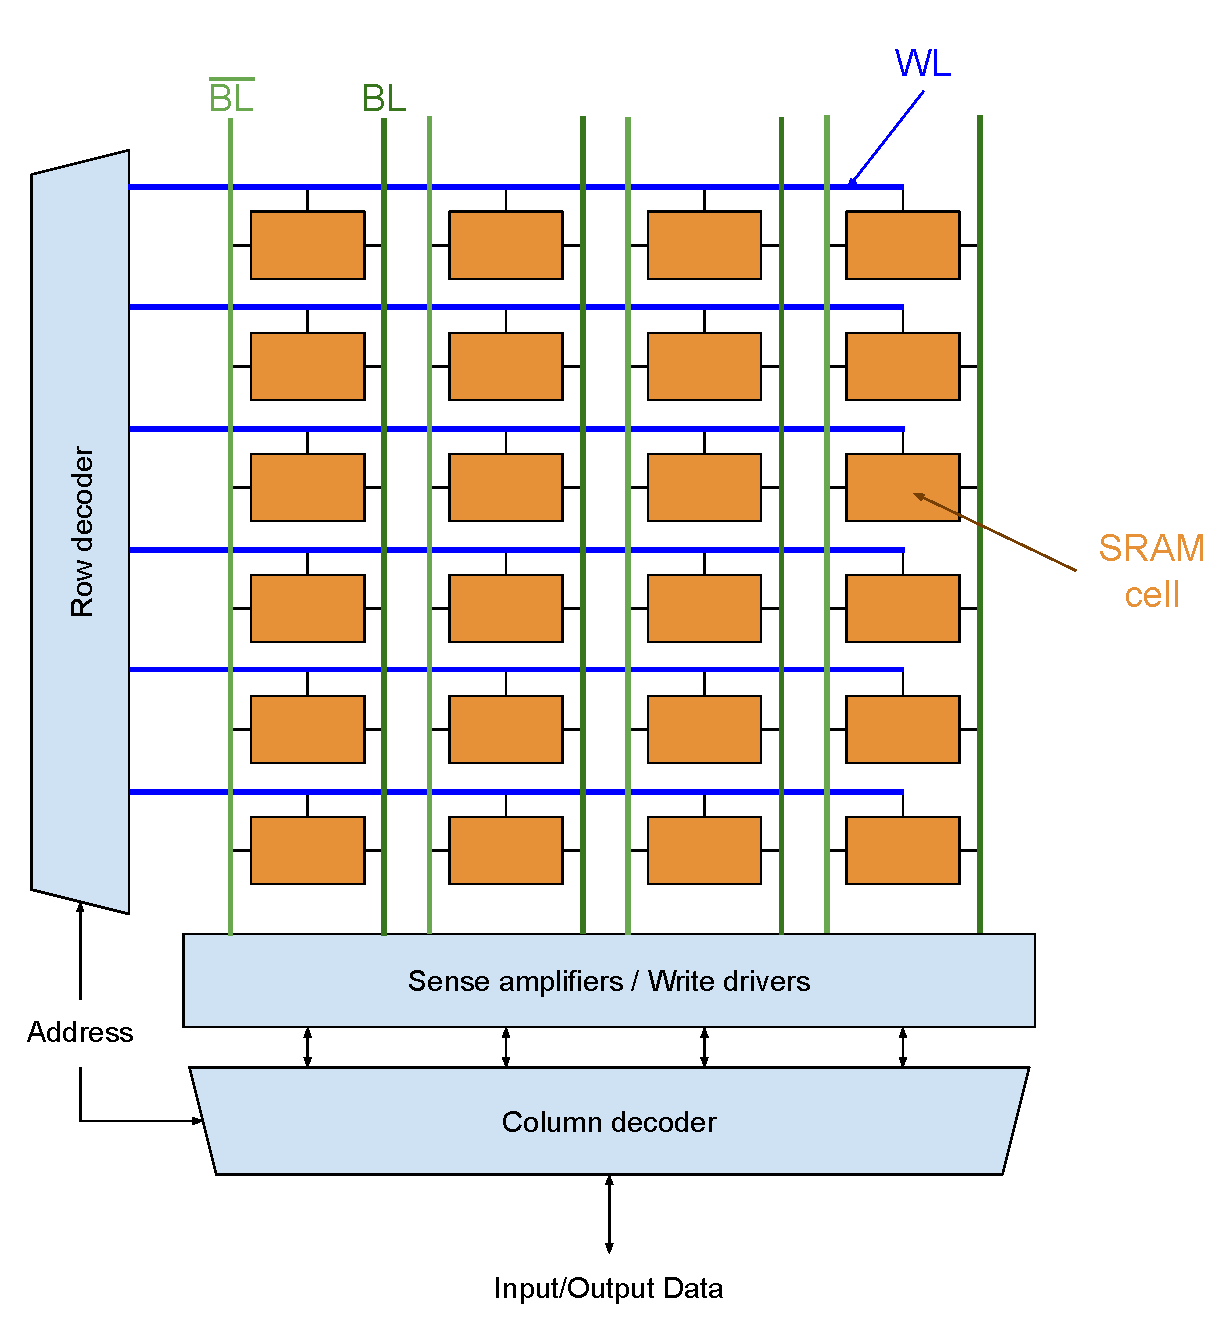
\includegraphics[width=11cm]{images/SRAM Architecture.pdf}
    \caption{A simple 4x6 SRAM array structure}
    \label{fig:SRAM_array}
\end{figure}

 Each individual cell is addressed by selecting the appropriate wordline and bitline pairs. As mentioned before, these ``lines'' are selected by the row decoder and the column decoder, respectively, setting the specified wordline high and connecting the pair of bitlines to the sense amplifiers for reading, or to the write drivers for writing. Sense amplifiers amplify a small differential voltage to a full swing digital output signal, the value of the selected cell. Write drivers control the voltage level during write operation to change the state of the cell to the provided input.  
 
 In the following section the topology of the SRAM 6T cell, which is the one used in this work, will be examined in detail, along with how the read and write operations are performed. 





\section{The SRAM 6T cell}

%More detailed description of SRAM PUFs along with a description of an SRAM cell. 4-5 Páginas


Although other designs exist, the standard topology for the SRAM cell is the 6T cell shown in fig. \ref{fig:SRAM}, which uses six transistors and is the cell generally employed in PUFs. 

\begin{figure}[H]
    \centering
    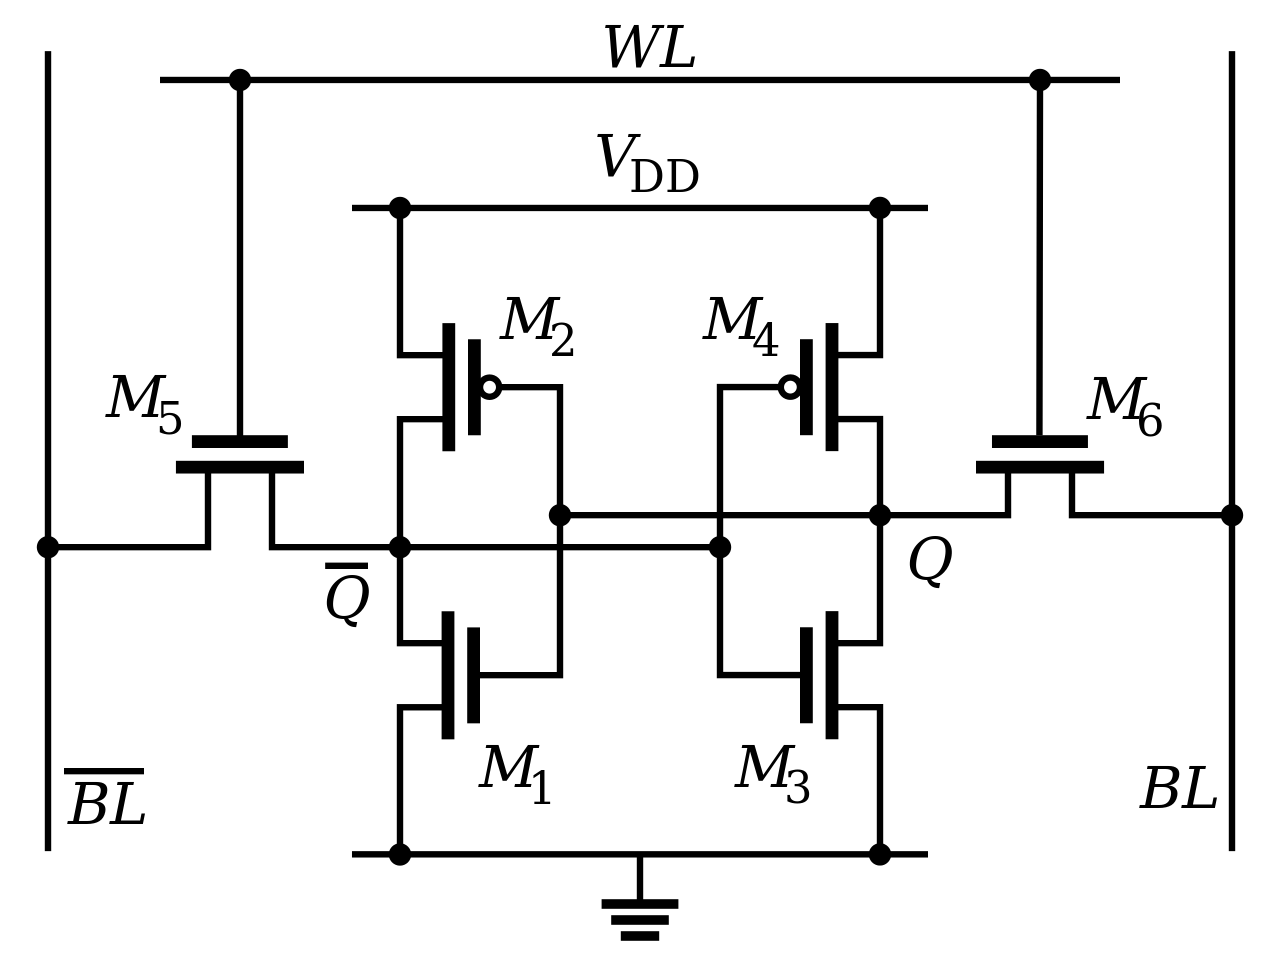
\includegraphics[width=9cm]{images/SRAM_Cell.png}
    \caption{Schematic of a 6T SRAM cell}
    \label{fig:SRAM}
\end{figure}

This cell is comprised of two cross-coupled inverters and two NMOS access transistors. The inverters set the voltage value of the internal nodes of the cell ($Q$ and $\overline{Q}$) through one pull-up (PMOS) and one pull-down (NMOS) transistor each. When the system is in a steady state, one of the nodes is at a high voltage ($V_{DD}$) and the other at a low voltage ($V_{SS}$ or ground). The values corresponding to $V_{DD}$ or $V_{SS}$ depend on the implementation. Accordingly, there are two possible states:

\begin{enumerate}
    \item $Q$ at high voltage and $\overline{Q}$ at low voltage.
    \item $Q$ at low voltage and $\overline{Q}$ at high voltage.
\end{enumerate}

One of the states represents the logic value 1 and the other 0. The choice is arbitrary but must be consistent. Without loss of generality due to the symmetry of the cell, from this point onward logic 1 corresponds to the first state and logic 0 to the second state. Positive feedback forces the cell into one of the two states. The SRAM cell has three modes of operation: holding, writing and reading. The access transistors isolate the cell from the circuit during holding to preserve the written value, and allow access during writing and reading. Access transistors are controlled by the wordline ($WL$) signal. The other connections to the cell are the bit line signals ($BL$ and $\overline{BL}$) which are connected to the internal nodes when the access transistors allow them. The bit line connection affects the internal nodes by introducing a small perturbation. This is useful for changing the state of the cell during the writing operation but must not be strong enough to change the state during the reading operation. These two modes of operation are examined now with more detail. 

\subsection*{Reading}

 To perform the reading, both bit-lines are first driven to the high voltage value, $V_{dd}$. Then, the $WL$ signal is activated. The process is illustrated in fig. \ref{fig:readwrite} (b). One internal node will be at a low voltage and the other at a high voltage. The bitline connected to the node at low voltage discharges slightly, while the other bitline stays at roughly the same voltage. This difference is measured by a sense amplifier. The stored value is determined depending on which one of the bitlines has the higher voltage. 

The internal node at low voltage rises its value as well when connected to the bitline. If this perturbation is small, the cell's feedback will be able to compensate once the reading is over. However, if it reaches a critical value it could alter the stored value and cause an error. The magnitude of this perturbation depends on the relative value between the width of the inverter's pull-down transistor ($M_1$ or $M_3$, depending on the state) and the width of the access transistors ($M_5$ and $M_6$ respectively). 

\begin{figure}[H]
    \centering
    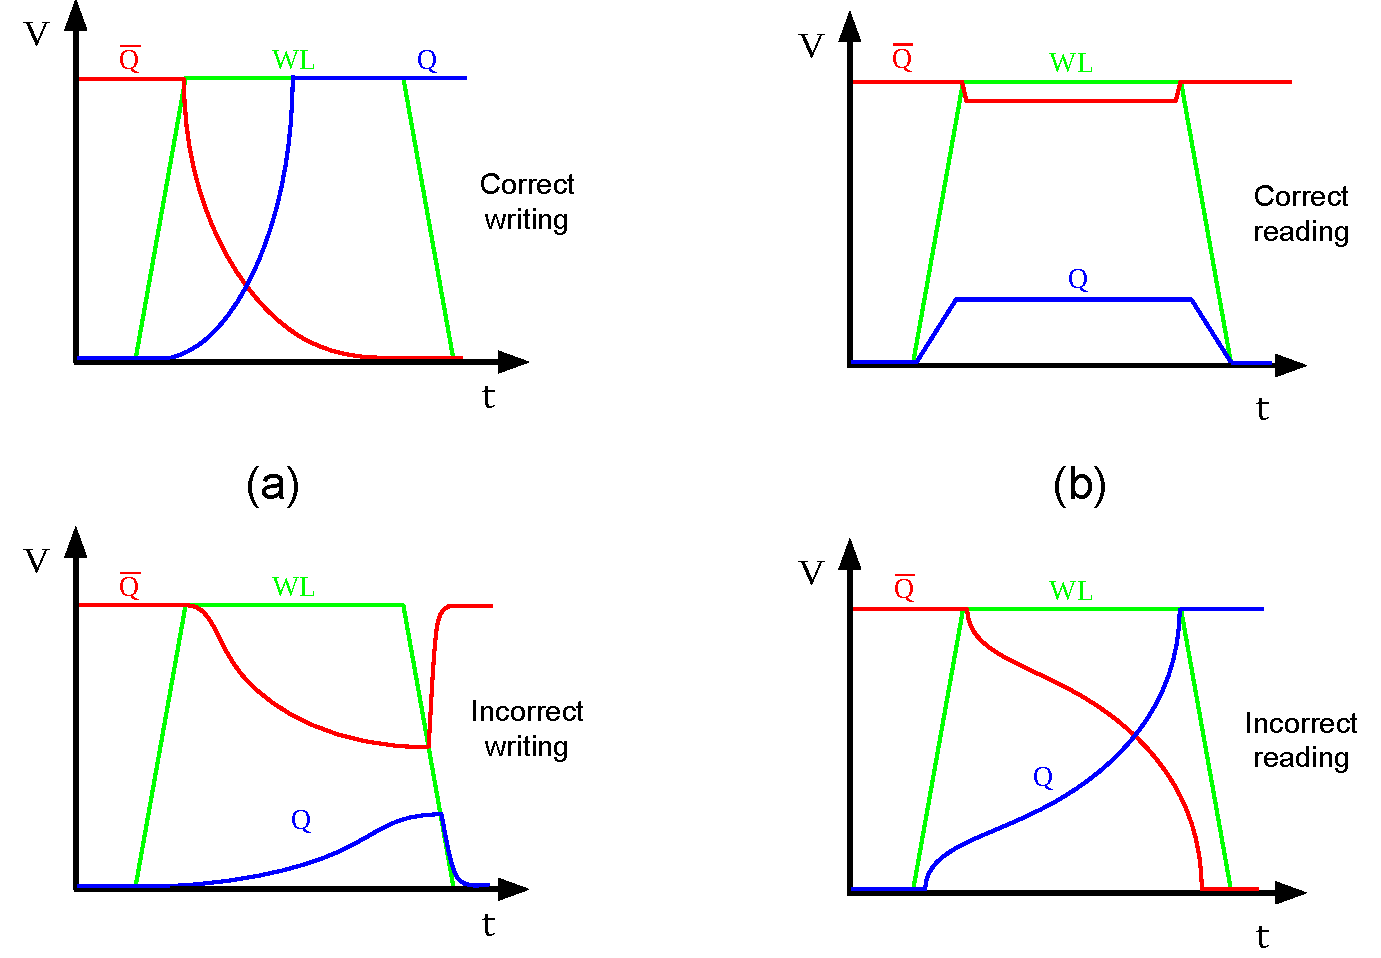
\includegraphics[width=15cm]{images/SRAM Read_Write.pdf}
    \caption{Voltage at the internal nodes and $WL$ signal during a successful and unsuccessful writing (a) and reading (b) operation. The starting state is $Q$ at low voltage and $\overline{Q}$ at high voltage, but the diagram would be similar for the other starting state. }
    \label{fig:readwrite}
\end{figure}

\subsection*{Writing}

This process is illustrated in fig. \ref{fig:readwrite} (b). To perform the writing, each bit-line is driven to the desired voltage values of their respective internal nodes through the write drivers. The objective when writing is to change the state of the cell. To accomplish that, the node at low voltage has to increase to high voltage, and vice versa. The $WL$ signal is then activated. The low voltage node increases its voltage at a rate which depends on the relative widths of the inverter's pull-up transistor ($M_2$ or $M_4$, depending on the state) and the width of the access transistors ($M_5$ and $M_6$ respectively). The high voltage node decreases its voltage at a rate which depends on the relative widths of the inverter's pull-down transistor ($M_1$ or $M_3$) and the width of the access transistors ($M_5$ and $M_6$ respectively). 

If the perturbance is not big enough, the voltage will not be flipped by the time the $WL$ signal is deactivated. In this case, the nodes will go back to their original state and the writing operation will have failed. Accordingly, the widths of the transistors must be tuned to have a perturbation strong enough for writing and weak enough for reading. 




\section{SRAM as a PUF}

An introduction to SRAM PUFs was provided in \ref{ss:cap2SRAM}. Since SRAM PUFs are the focus on this work, a more detailed look into them is required. As explained before, SRAM PUFs exploit the mismatch due to fabrication process variability between the two inverters by measuring the start-up value of SRAM cells, determined by which one of the two inverters powers up faster. 

Whether one inverter or the other powers up faster depends on the threshold voltage $V_{th}$ of the different transistors. In order to simply illustrate this, we will consider that the strength of the cell depends only on the $V_{th}$ values of the PMOS transistors $M_2$ and $M_4$ (using fig. \ref{fig:SRAM} as reference). As an example, suppose that mismatch causes $|V_{th2}|$ to be smaller than $|V_{th4}|$. When the cell powers up, i.e. $V_{dd}$ rises, $M_2$ will start conducting before $M_4$, causing $\overline{Q}$ to go up to high voltage and $Q$ to low voltage, resulting in a power-up state of ``0'' by the criteria defined earlier.   

 Generalizing this example, if the difference between threshold voltages is $\Delta V_{th}=|V_{th2}|-|V_{th4}|$ the cell should power up to ``1'' for $\Delta V_{th}>0$ and to ``0'' for $\Delta V_{th}<0$. However, some cells (below 20\%) with $|V_{th2}|\approx|V_{th4}|$ may change their power-up values when this is determined at different moments, due to operating temperature differences, supply voltage variations, aging or noise \cite{Baturone2015}. These are considered unstable and are largely responsible for the bit flips in the SRAM response. Most cells (above 80\%) have a large enough difference to reliably power-up to the same state and are considered stable.
 
 Figure \ref{fig:celldistribution} illustrates this if the distribution of the transistors' threshold voltage is assumed to be gaussian as in the mismatch models \cite{Hofer2010}. Cells with values in the middle region are considered unstable, shown in red. The bias does not have to be very strong to have a stable cell; so, generally, a majority of cells are considered stable, shown in light green. 

\begin{figure}[t]
    \centering
    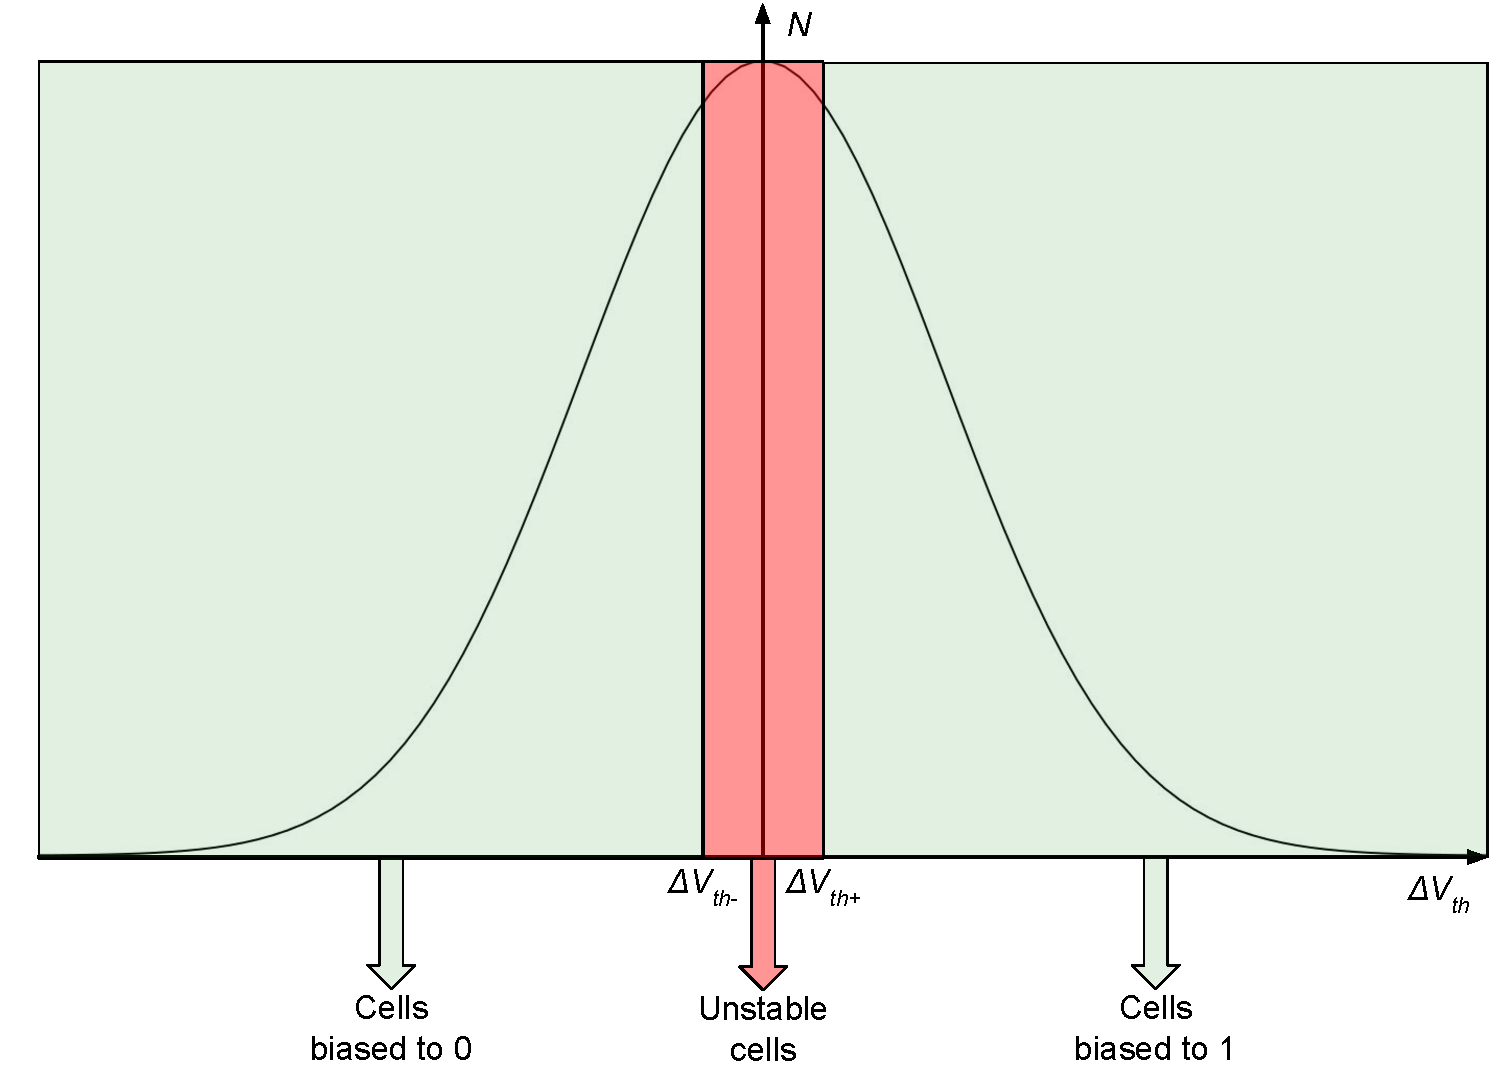
\includegraphics[width=14cm]{images/Cell distribution.pdf}
    \caption{Number of cells $N$ corresponding to a certain value of $\Delta V_{th}$. Cells with $\Delta V_{th} \approx 0 $ are unstable, while those to the left are biased to zero and those to the right to one.}
    \label{fig:celldistribution}
\end{figure}


Although only the mismatch of the PMOS transistors was considered regarding the power-up state of the cell, the mismatch of the NMOS transistors is important as well. The NMOS transistor that starts conducting faster pulls its node to low voltage, as they are connected to $V_{ss}$. Their contribution depends on how fast the SRAM powers up \cite{Wang2018}, i.e. the power supply ramp rate. This contribution ranges from NMOS mismatch having almost no impact for near instant power-ups (1 ns) to NMOS mismatch having the same impact as PMOS for slow power-ups (1 s). In the second case, $\Delta V_{th}$ is calculated as $\Delta V_{th}=|V_{th2}|+|V_{th3}|-|V_{th4}|-|V_{th1}|$. 
In essence, depending on the difference in threshold voltages the cell will have more or less reliability working as a PUF. It is important to keep in mind that the stable cells still have some degree of unreliability over a large enough number of power-ups \cite{Liu2017}.

The standard solution for unstable cells in the context of PUFs used for key generation is employing helper data algorithms, but the requirements of heavy ECCs are quite costly as described in the previous chapter. Some proposed SRAM bit selection techniques which attempt to select only stable cells are evaluated in the next chapter. If the unstable cells are separated from the stable ones, they can still be useful for entropy generation \cite{Baturone2015}. 

Other approaches specific to SRAM PUFs have been studied to reduce this problem \cite{Baturone2015}. For example, in \cite{Okumura2011,Hofer2010,Shifman2018} they use a custom design of the SRAM cell. Specifically, in \cite{Okumura2011} write drivers and PMOS switches are added to the SRAM cell, in \cite{Hofer2010} circuitry to measure the threshold voltage is added so that only stable cells are used and in \cite{Shifman2018} the power supply of each inverter is routed independently to perform small independent variations and select stable cells based on their response to those variations and a Miller capacitor is added to increase stability. However, these methods are costly and renounce to one of the main advantages of SRAM PUFs, the ability to use generic SRAM cells already present in ICs. 

\section{Sources of reliability degradation}

It is important as well to characterize how local temperature differences, supply voltage variations and aging affect PUF reliability. An overview is provided in the following subsections. From this understanding the reliability of the SRAM PUF can be properly measured and new techniques to boost reliability can be developed and tested.

 
\subsection{Supply voltage}


SRAM cells power up by rising their supply voltage from zero to $V_{dd}$. There are two different aspects concerning supply voltage and reliability.

On the one hand, possible deviations from the nominal value of supply voltage $V_{dd}$. This is usually tested by evaluating the circuit at supply voltages of $\pm 10 \%$ of the nominal supply voltage \cite{Schrijen2012}. However, the start-up value of the cell should be established during power-up and the supply level at the end of the ramp should not have a large impact on SRAM PUF reliability.

On the other hand, the ramp-up time has a pronounced effect on reliability \cite{Claes2012,Wang2018}. There is a wide range to choose from, from the order of $\mu s$ to around one second. The issue is that faster ramps are better for high temperatures while slower ramps are better for low temperatures \cite{Cortez2013}. According to this, in \cite{Cortez2013} a proposal to dynamically change the ramp-up time is made. In any case, the effects vary according to the device design and a careful choice based on experimental data must be made to achieve optimal reliability. 


\subsection{Temperature}

Temperature is quite influential on the performance of ICs. In SRAM PUFs it directly affects the characteristics of transistors, and, therefore, the PUF response \cite{Schrijen2012}. Accordingly, it is of great importance to properly characterize its effects for reliability. This is done by measuring the behaviour of the chip in a certain temperature range. These ranges depend on the implementation. Although the specific range may vary, generally accepted ones are \cite{operating_temperature}:

\begin{itemize}
    \item Commercial: $0\degree \mathrm{C}$ to $70\degree \mathrm{C}$
    \item Industrial: $-40\degree \mathrm{C}$ to $85\degree \mathrm{C}$
    \item Military: $-55\degree \mathrm{C}$ to $125\degree \mathrm{C}$
\end{itemize}

Usually, PUFs are tested in the industrial range \cite{VanDerLeest2012,Schrijen2012,Cortez2013}. Depending on the SRAM design, the worst case reliability can be in either extreme of the temperature range \cite{Schrijen2012}. 

\subsection{Aging}
\label{sec:aging}
%Causes of aging in SRAM (BTI, HCI, RTN). Models of aging developed. 5-6 páginas

As technology scaling continues in microelectronics, SRAM cells become smaller and time dependent degradation of electrical properties (aging) becomes more severe. Understanding aging is important to predict errors in any electronic implementation. 

%This is employed in \cite{Garg2014,Mispan2016,Bhargava2013}.

Aging can have a wide range of effects, from a change in threshold voltage, and the consequent increase in delay times, to permanent failure. Naturally, the change in threshold voltage is very important in SRAM PUFs since it may change the bias of one cell from one state to another during power-up. Aging depends in more variables than just time, being influenced by workload during operation, environmental conditions and electrical stress. 

%Electrical stress implies supply voltage levels higher than the nominal value of  $V_{dd}$.To accelerate aging a useful and common technique is to apply high electrical stress for short periods of time, trying to emulate a degradation similar to years of operation under nominal conditions \cite{Maes2014}. An SRAM PUF aged this way provides an estimation on the worst case reliability regarding aging. 

 The aging mechanisms generally considered for SRAM cells are Bias Temperature Instability (BTI), Hot-Carrier Injection (HCI), Time-Dependent Dielectric Breakdown (TDDB) and Electromigration (EM) \cite{Kraak2018}. BTI, HCI and TDDB occur in the gate oxides of transistors while EM happens in the interconnect metal lines. BTI and HCI are the main concern regarding PUF reliability as they occur at nominal voltages. More studies have been performed for BTI than HCI but an exact model for either one has not yet been created \cite{Schlunder2012}. In the subsequent subsections the effects of BTI and HCI will be considered qualitatively. 


\subsubsection{BTI}

BTI includes NBTI (Negative-Bias Temperature Instability) effects, which occur in PMOS transistors, and PBTI (Positive-Bias Temperature Instability) effects, which occur in NMOS transistors. NBTI is generally dominant over PBTI for small technology nodes \cite{Kraak2018} and consequently NBTI aging is the main focus of study. NBTI increases the threshold voltage of the transistors and the consequent decrease in drain current and transconductance. It is caused by positive charges built up in the MOS gate insulator due to the application of negative gate bias. There is no consensus on a model for NBTI \cite{Stathis2018}. The Reaction-Diffusion model holds that NBTI is a diffusion-limited process and the Defect-Centric model holds that it is reaction-limited. According to the first one, interface traps are generated during operation and these interface states become positively charged when the PMOS device is biased in the "on" state, i.e. with negative gate voltage. According to the second one, preexisting traps located in the bulk of the dielectric are filled with holes coming from the channel of PMOS.

Either the oxide electric field caused by negative gate voltages or elevated temperatures can produce NBTI, but a stronger and faster effect is produced by their combined action. Due to technology scaling, the magnitude of the electric field becomes greater, so NBTI is always going to be present and will be stronger as scaling keeps progressing \cite{Schroder2003}. This degradation phenomenon reveals a stochastic and discrete nature for technology nodes in the nanometer range, which means that identical transistors (and therefore circuits) may age differently \cite{Kaczer2010}. The effects of NBTI have a permanent and a temporal component, since part of the degradation can be recovered over time when stress is removed (i.e. when the gate voltage is removed). 

%Some of these include guard-banding, gate-sizing and voltage tuning. Differential structures will make the stress less noticeable as well \cite{Lee_aging_techniques}.

How does BTI affect an SRAM cell? The 6-T standard cell shown in fig. \ref{fig:SRAM} is considered. Suppose it is biased so that $Q$ is at the high voltage at power up. This corresponds to a state 1 according to the criteria expressed earlier. Accordingly, the left NMOS transistor has a smaller threshold voltage than its pair and/or the right PMOS transistor has a smaller threshold voltage than its pair. They will be the first to turn ON and will make the cell take the 1 logic value due to the feedback. If node $Q$ is at a high voltage following the nomenclature of fig. \ref{fig:SRAM} the NMOS transistor $M_3$ will be off and the PMOS transistor $M_1$ will be on and suffering PBTI.  On the other hand, node $Q$ will be at a low voltage, so PMOS transistor $M_4$ will be off and the NMOS transistor $M_2$ will be on and suffering PBTI. NBTI occurs in the PMOS transistor, so this transistor will be more affected. In any case, threshold voltage increases over time, consequently reducing the initial bias of the cell. The reasoning is the same if the cell is biased towards 0. If the cell is written to its non preferred value, BTI will instead increase the existing bias. 

If the initial power-up bias of a cell is reduced over time, stable cells will turn unstable progressively. However, it can be solved by storing the non preferred value in the cell, which mitigates the stress caused during functional operation. This technique, called directed accelerated aging (DAA) \cite{Roelke2018}, can be used to increase the initial bias and the resulting reliability of the cell. It can even be used to flip the initial skew of a cell and make it strongly biased to the other state. This is used in \cite{Garg2014} to improve the uniformity of the PUF response as well. 

%In \cite{Maes2012} a SRAM PUF is shown to have an increase of about 2\% in terms of Bit Error Rate after 4.5 years of operation based on experimental results where accelerated aging was applied. 


\subsubsection{HCI}

HCI is a phenomenon by which the threshold voltage of a transistor is altered when high energy carriers are trapped in the gate oxide, as in BTI. However, HCI is caused by a flowing drain current, in which moving charge carriers (the hot carriers) break up the bonds between silicon and hydrogen at the boundary between the transistor channel and gate dielectric. The carriers need a certain kinetic energy to achieve this. When velocity saturates, electron's average velocity will not increase but the random kinetic energy of some electrons can achieve the required kinetic energy to break the silicon-oxide barrier due to random collisions. Once electrons start to break the barrier, a small leakage current appears and traps can occur.

The requirements for HCI to be present are high electric fields and long mean free path, i.e. the average distance travelled by an electron between collisions. As in BTI effects, technology scaling makes high electric fields common. Increasing the voltage will make degradation more pronounced. On the other hand, the mean free path for electrons to be accelerated is inversely proportional to temperature, so lower temperatures will increase HCI. In digital gates, it occurs only when the device switches, so the effect is proportional to the signal activity factor (ratio of average number of signal transitions to clock transitions and the clock frequency) \cite{Sengupta2017}.  The  recoverable component of HCI degradation is very small compared to BTI \cite{Bhargava2013}, so HCI has high permanence (does not lessen significantly over time).

Although BTI degradation is the most popular for DAA in the literature, in \cite{Bhargava2013} HCI is used to boost reliability by applying stress through a $V_{DS}$ increase. The advantages over BTI are shorter stress time, high permanence and requiring only a one-time reinforcement stress. 

% \subsection{TDDB}



% \subsection{EM}

% Electromigration is the transport of conductive material in the direction of the current caused by the momenta exchange between current carrying electrons and the conductor's metal lattice. The effect is proportional to current density, so miniaturization increases it as well. The main consequence is the eventual loss of connections or failure in a circuit. However, proper design practices consider the effects of electromigration \cite{Lienig2018}. These practices are generally incorporated in the automated design tools. Electromigration has been known and studied for a long time and is relatively predictable, so it isn't a major concern for SRAM PUFs in their usual lifespan.








